\begin{ex}
	\begin{condition}
		\begin{minipage}[t]{0.67\textwidth}
			На рисунке изображён график функции \( y = f'(x) \) - производной функции
			\( f(х) \), определенной на интервале \( ( -5; 5) \). Найдите точку минимума функции \( f(x) \).\answer{?}
		\end{minipage}
		\begin{minipage}[c]{0.25\textwidth}
			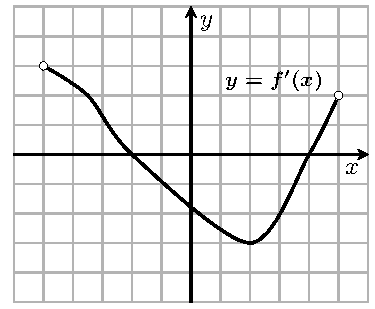
\includegraphics[align=t, width=\textwidth]{graphs/graph_0/graph_0}
		\end{minipage}
	\end{condition}
\end{ex}